\section{Introduction}\label{sec:introduction}

Large language models (LLMs) have shown impressive reasoning abilities in handling complex tasks \citep{qiao2023reasoning,huang2023towards}, marking a significant leap that bridges the gap between human and machine intelligence. However, LLMs still struggle with conducting faithful reasoning due to issues of \emph{lack of knowledge} and \emph{hallucination} \citep{huanglarge,wang2023knowledge}. These issues result in factual errors and flawed reasoning processes \citep{nguyen-etal-2024-direct}, which greatly undermine the reliability of LLMs in real-world applications.

To address these issues, many studies utilize knowledge graphs (KGs), which encapsulate extensive factual information in a structured format, to improve the reasoning abilities of LLMs \citep{pan2023unifying,luo2024rog}. Nevertheless, because of the unstructured nature of LLMs, directly applying them to reason on KGs is challenging.

% Following can be removed if space is limited
Existing KG-enhanced LLM reasoning methods can be roughly categorized into two groups: \emph{retrieval-based} and \emph{agent-based} paradigms, as shown in \Cref{fig:framework} (a) and (b). Retrieval-based methods \citep{li2023graph,yang2024kg,dehghan-etal-2024-ewek} retrieve relevant facts from KGs with an external retriever and then feed them into the inputs of LLMs for reasoning. Agent-based methods \citep{sunthink,zhu2024knowagent,jiang2024kg} treat LLMs as agents that iteratively interact with KGs to find reasoning paths and answers.

\begin{wrapfigure}{r}{0.4\columnwidth}
    \vspace{-30pt}
    \begin{center}
        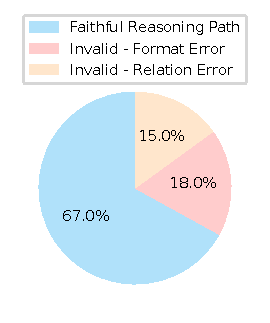
\includegraphics[width=0.4\columnwidth,trim=0.4cm 0.6cm 0.4cm 0.2cm,clip]{images/hallucination_ratio.pdf}
      \end{center}
      \vspace{-15pt}
      \caption{Analysis of reasoning errors in RoG \citep{luo2024rog}.}
      \vspace{-15pt}
    \label{fig:hallucination_ratio}
\end{wrapfigure}
Despite their success, retrieval-based methods require additional accurate retrievers, which may not generalize well to unseen questions or account for the graph structure \citep{mavromatis2024gnn}. Conversely, agent-based methods necessitate multiple rounds of interaction between agents and KGs, leading to high computational costs and latency \citep{dehghan-etal-2024-ewek}. Furthermore, existing works still suffer from serious hallucination issues \citep{agrawal2024mindful}. \citet{sui2024fidelis} indicates that RoG \citep{luo2024rog}, a leading KG-enhanced reasoning method, still experiences 33\% hallucination errors during reasoning on KGs, as shown in \Cref{fig:hallucination_ratio}.


To this end, we introduce graph-constrained reasoning (\ourmethod), a novel KG-guided reasoning paradigm that connects unstructured reasoning in LLMs with structured knowledge in KGs, seeking to eliminate hallucinations during reasoning on KGs and ensure faithful reasoning. Inspired by the concept that LLMs reason through decoding \citep{wei2022chain}, we incorporate the KG structure into the LLM decoding process. This enables LLMs to directly reason on graphs by generating reliable reasoning paths grounded in KGs that lead to correct answers.

In \ourmethod, we first convert KG into a structured index, KG-Trie, to facilitate efficient reasoning on KG using LLM. Trie is also known as the prefix tree \citep{wiki:trie} that compresses a set of strings, which can be used to restrict LLM output tokens to those starting with valid prefixes \citep{deautoregressive,xie2022discrimination}. KG-Trie encodes the reasoning paths in KGs as formatted strings to constrain the decoding process of LLMs. Then, we propose graph-constrained decoding that employs a lightweight KG-specialized LLM to generate multiple KG-grounded reasoning paths and hypothesis answers. With the constraints from KG-Trie, we ensure faithful reasoning while leveraging the strong reasoning capabilities of LLMs to efficiently explore paths on KGs in constant time. Finally, we input multiple generated reasoning paths and hypothesis answers into a powerful general LLM to utilize its inductive reasoning ability to produce final answers. In this way, \ourmethod combines the graph reasoning strength of KG-specialized LLMs and the inductive reasoning advantage in general LLMs to achieve faithful and accurate reasoning on KGs.
%
The main contributions of this work are as follows:
\begin{itemize}
    \item We propose a novel framework called graph-constrained reasoning (\ourmethod) that bridges the gap between structured knowledge in KGs and unstructured reasoning in LLMs, allowing for efficient reasoning on KGs via LLM decoding.
    \item We combine the complementary strengths of a lightweight KG-specialized LLM with a powerful general LLM to enhance reasoning performance by leveraging their respective graph-based reasoning and inductive reasoning capabilities.
    \item We conduct extensive experiments on several KGQA reasoning benchmarks, demonstrating that \ourmethod not only achieves state-of-the-art performance with zero hallucination, but also shows zero-shot generalizability for reasoning on unseen KGs without additional training.
\end{itemize}